\section{Agent-based Model}
In this section, we provide a formal description of \href{https://github.com/InstituteforDiseaseModeling/covasim}{covasim} model \citep{kerr2021covasim} and how we model vaccinations, mask policies and mobility changes within our model.
\subsection{Disease progression}
\begin{figure}
	\centering
	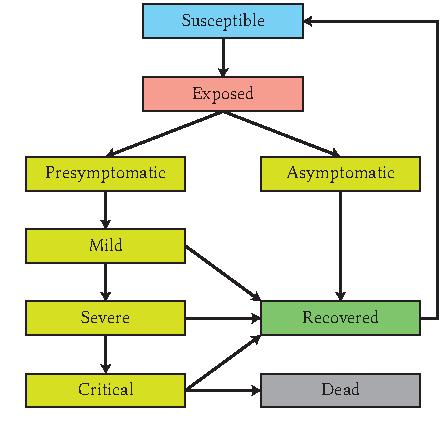
\includegraphics{model/seir.pdf}
	\caption{Covasim model, disease state transformation structure}
	\label{seir}
\end{figure}

In covasim, the disease state of an agent is characterized as susceptible, exposed, infectious (asymptomatic, presymptomatic, mild, severe, critical), recovered and dead. The Figure \ref{seir} shows all possible transformation between any two disease states. Each transformation is also parameterized with a probability $p$ (how likely does the transformation happen) and a duration $\tau$ (how long does the transformation take). The age-linked value of $p$ and the distribution of $\tau$ are detrived from lots of previous research and are built in \href{https://github.com/InstituteforDiseaseModeling/covasim}{covasim}.

\subsection{Contact network}

To model the contact network between people, covasim assigns people to four network layers: household, school, workplace and community. More specifically, covasim generates a population of people based on the location-specific age distribution. After that, covasim assigns people aged between 6 and 22 to schools, assigns people aged between 22 and 65 to workplaces and assigns people to households based on the location-specific household size.

Within each network, the contact number of each person is sampled from poisson distributions. For each contact between a susceptible individual and an infectious individual, the probability of a successful virus transmission is $\beta$.

\subsection{Agent states}

One important feature of covasim is that it provides several useful agent states so that it can describe testing, contact-tracing, quarantine and isolation policies. Figure \ref{state} lists out built in agent states and transformations between them.
\begin{itemize}
	\item Free: If an agent is free, the agent has $100\%~\beta$ value. If a free agent has a contact with a confirmed case and is traced successfully, the agent will become quarantined. If a free agent has positive test results, the agent will become isolated.
	\item Quarantined: If an agent is quarantined, the agent has $60\%~\beta$ in the household layer and $20\%~\beta$ in other layers. The quarantine ends when it reaches the maximum quarantine time. However, if a quarantined agent has positive test results, the agent will also get isolated.
	\item Isolated: If an agent is isolated, the agent has $30\%~\beta$ in the household layer and $10\%~\beta$ in other layers. A isolated agent will become free once the agent recovers.
\end{itemize}

\begin{figure}
	\centering
	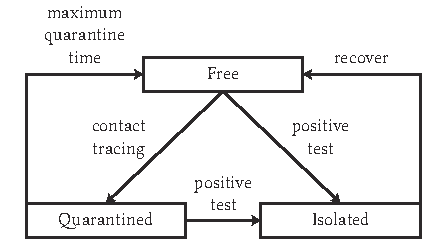
\includegraphics{model/state.pdf}
	\caption{Covasim model, agent state transformation structure}
	\label{state}
\end{figure}

\subsection{Mask policies and mobility}
There are two important factors which affect the spread of COVID-19. The first one is personal protection, such as wearing masks, washing hands, etc, which reduces the probability of virus transmission per contact, i.e., the $\beta$ value The second one is social distancing, such as avoiding crowds, keeping distance from others, staying at home, etc, which reduces the contact number of each agent.

Within our model, we use mask policies and mobility to represent personal protection and social distancing respectively. More specifically, denote numerical mask policies and mobility as $x_{\text{ma}},x_{\text{mo}}$, we define a function $f:\mathcal{R}^2\rightarrow[0,1]$ as:
\begin{equation}
	f(x_{\text{ma}},x_{\text{mo}})=\frac{2(a_1x_{\text{ma}}+b_1)(a_2x_{\text{mo}}+b_2)}{(a_1x_{\text{ma}}+b_1)+(a_2x_{\text{mo}}+b_2)}
\end{equation}

We can view this function as first applying two linear transformation on $x_1=a_1x_{\text{ma}}+b_1$, $x_2=a_2x_{\text{mo}}+b_2$ and then apply the function $g(x_1,x_2)=2x_1x_2/(x_1+x_2)$. We can view the function $g$ in another way:

\begin{equation}
    \begin{split}
         g&(x_1,x_2)=\frac{2x_1x_2}{x_1+x_2}\\
         &=\min\{x_1,x_2\}\frac{\max\{x_1,x_2\}}{x_1+x_2} + \max\{x_1,x_2\}\frac{\min\{x_1,x_2\}}{x_1+x_2}
    \end{split}
\end{equation}

We design such function because we believe that the smaller value of $x_1,x_2$ has a larger impact of $\beta$. After that, for each day we calculate the $\beta$ value as $f(x_{\text{ma}},x_{\text{mo}})\beta_0$, where the $\beta_0$ is a constant within one outbreak (for a variant of SARS-CoV-2) and $x_{\text{ma}},x_{\text{mo}}$ changes each day.
